% !TeX spellcheck = fr_FR

% TODO: Replace scan images with clean text where possible

\documentclass[a4paper, 10pt]{report}

\usepackage[french]{babel}
\usepackage[T1]{fontenc}

\usepackage{amsmath, amssymb, amsfonts}

\usepackage{hyperref}
\usepackage{geometry}

\usepackage{xcolor}
\usepackage{graphicx}

\usepackage{fancyhdr}
\usepackage{lastpage}

\usepackage{enumitem}

\geometry{
	a4paper,
	left=25mm,
	right=25mm,
	top=35mm,
	bottom=25mm,
	headsep=5mm,
	headheight=20mm,
}

\definecolor{solution}{HTML}{E5E4E2}
\providecommand{\abs}[1]{\lvert#1\rvert}
\providecommand{\norm}[1]{\lVert#1\rVert}
\DeclareMathOperator{\card}{card}

\begin{document}
	
	\renewcommand{\headrule}{%
		\vspace{-4pt}\hrulefill
		\raisebox{-6.8pt}{\ 
\includegraphics[height=5mm]{../../icon.png}}
		\hrulefill
	}	
	\pagestyle{fancy}
	\fancyhf{}
	
	\fancyhead[L]{\small \slshape Automne 2024}
	\fancyhead[C]{\Large \bfseries Analyse I - Série 04}
	\fancyhead[R]{\small Buff Mathias}
	\fancyfoot[L]{
		\small Source files available at:
		\href{https://github.com/MathiasBuff/bsc-math}
		{github.com/MathiasBuff/bsc-math}
	}
	\fancyfoot[R]{
		\small Page \thepage
		\hspace{1pt} /
		\pageref*{LastPage}
	}
	

	\noindent
	\textbf{Exercice 1.} Montrer par récurrence que
	\begin{enumerate}[label=(\roman*)]
		\item $\displaystyle\sum_{k=0}^{n} k = \frac{n(n+1)}{2}$
		pour tout $n \in \mathbb{N}$
		%
		\item $\displaystyle\sum_{k=0}^{n} k^3 = 
			\left(\frac{n(n+1)}{2}\right)^2$
		pour tout $n \in \mathbb{N}$
		%
		\item $\displaystyle\sum_{k=0}^{n} a^k = \frac{1 - a^{n+1}}{1 -a}$
		pour tout $a \neq 1$ et $n \in \mathbb{N}$
	\end{enumerate}
	
	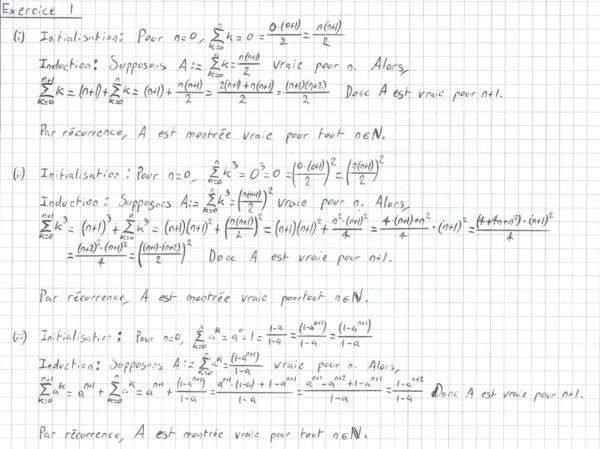
\includegraphics{ex01.jpg}
	
	\vspace{5mm}
	\noindent
	\textbf{Exercice 2.} Montrer par récurrence que pour tout
	$n \in \mathbb{N}$ on a  $n < 2^n$.
	
	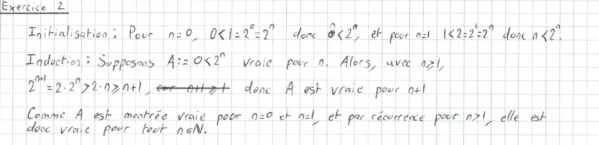
\includegraphics{ex02.jpg}	
	
	\newpage
	
	\fancyhf{}
	\renewcommand{\headrule}
	{\rule{\textwidth}{0pt}}
	\fancyfoot[R]{
		\small Page \thepage
		\hspace{1pt} /
		\pageref*{LastPage}
	}
	
	\noindent
	\textbf{Exercice 3.} Où est la faute de raisonnement dans la preuve
	suivante ? \\
	"Montrons que le plus grand entier naturel strictement positif est 1.\\
	En effet, soit $n$ le plus grand entier positif. Comme $n \geq 1$, nous
	trouvons $n^2 \geq n$. Mais puisque $n$ est le plus grand entier
	naturel, $n^2 \leq n$ de sorte que $n^2 = n$ et donc $n = 1$
	(puisque $n \neq 0$).\\
	Donc 1 est le plus grand entier naturel strictement positif."
	
	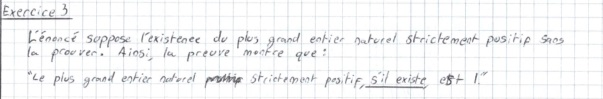
\includegraphics{ex03.jpg}
	
	\vspace{5mm}
	\noindent
	\textbf{Exercice 4.} (Inégalité de Bernoulli)\\
	Montrer par récurrence que pour tout $x \geq -1$ et tout
	$n \in \mathbb{N}$ on a $(1 + x)^n \geq 1 + nx$.
	
	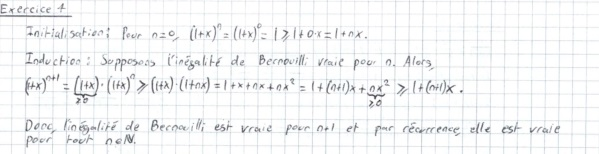
\includegraphics{ex04.jpg}
	
	\newpage
	
	\noindent
	\textbf{Exercice 5.} Trouver le supremum et l'infimum pour chacun des
	ensembles suivants.\\
	Préciser lorsqu'il s'agit d'un maximum ou d'un minimum.
	Justifier chaque réponse.
	\begin{enumerate}[label=(\roman*)]
		\item $[2, 3)$
		\item $[2, 3]$
		\item $(2, 3)$
		\item $(2, 3]$
		\item $[-2, 2] \cup (5, 8)$
		\item $[0,1] + [-3, 7] = \{x + y : x \in [0,1], y \in [-3,7]\}$
		\item $\{\frac{1}{n} : n \in \mathbb{N}^*\}$
		\item $\{x^2 : x \in [-1, 4)\}$
		\item $\{4 + \frac{1 + (-1)^n}{n} : n \in \mathbb{N}^*\}$
	\end{enumerate}
	
	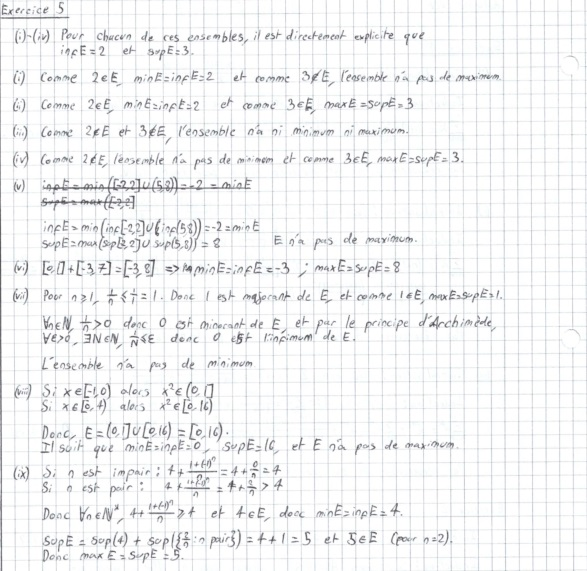
\includegraphics{ex05.jpg}
	
	\newpage
	
	\noindent
	\textbf{Exercice 6.} (Proposition 2.4)
	Montrer que pour tout $x, y \in \mathbb{R}$ on a
	\begin{enumerate}[label=(\roman*)]
		\item $\abs{x} = 0 \iff x = 0$
		\item $\abs{x \cdot y} = \abs{x} \cdot \abs{y}$
	\end{enumerate}
	
	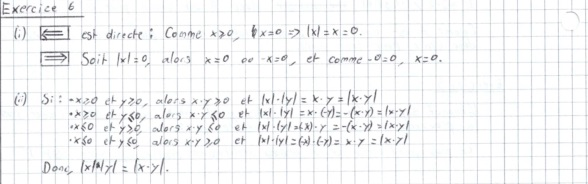
\includegraphics{ex06.jpg}
	
	\vspace{5mm}
	\noindent
	\textbf{Exercice 7.} Trouver $a$ et $b$ tels que
	$\frac{1}{k(k+1)} = \frac{a}{k} + \frac{b}{k+1}$.
	En déduire ce que vaut
	\[
		\sum_{k=1}^{n} \frac{1}{k(k+1)}
	\]
	
	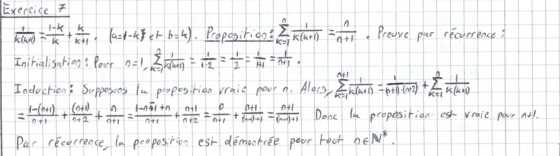
\includegraphics{ex07.jpg}
	
	\newpage
	
	\noindent
	\textbf{Exercice 8.} (Formule du binôme)\\
	Pour $p, n \in \mathbb{N}$ satisfaisant $0 \leq p \leq n$ on définit
	le coefficient binomial
	\[\begin{pmatrix}n\\p\end{pmatrix} = \frac{n!}{p!(n - p)!}\]
	(On utilise la convention habituelle $0! := 1$).
	\begin{enumerate}[label=(\roman*)]
		\item Pour $p < n$ montrer que
		\[
			\begin{pmatrix}n+1\\p+1\end{pmatrix} =
			\begin{pmatrix}n\\p\end{pmatrix} +
			\begin{pmatrix}n\\p+1\end{pmatrix}
		\]
		\item Montrer par récurrence la \textit{formule du binôme} : Pour
		tout $a, b \in \mathbb{R}$ et $n \in \mathbb{N}$ on a
		\[
			(a + b)^n = 
			\sum_{k=0}^{n} \begin{pmatrix}n\\k\end{pmatrix} a^k b^{n-k}
		\]
	\end{enumerate}
	
	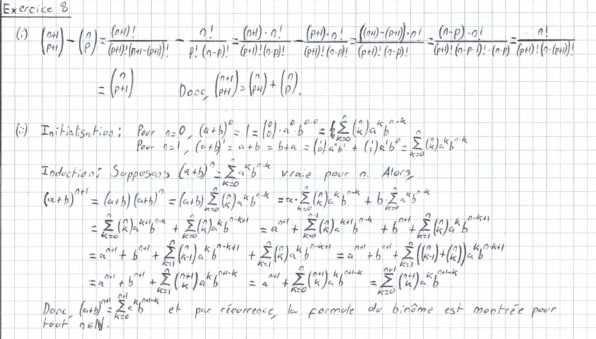
\includegraphics{ex08.jpg}
	
	\newpage
	
	\noindent
	\textbf{Exercice 9.}  Soient $A, B \subset \mathbb{R}$ et définissons
	\[
		A + B = \{x + y : x \in A, y \in B\},
		\quad
		A \cdot B = \{x \cdot y : x \in A, y \in B\}
	\]
	Montrer que $\sup(A+B) = \sup A + \sup B$.\\
	Quelle hypothèse faut-il rajouter à $A, B$ pour qu'on ait
	$\sup(A \cdot B) = \sup A \cdot \sup B$ ?
	
	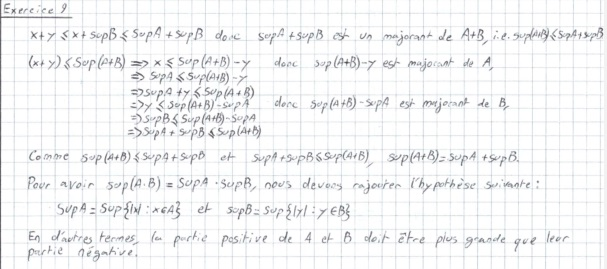
\includegraphics{ex09.jpg}
	
	\vspace{5mm}
	\noindent
	\textbf{Exercice 10.} Montrer que
	$\displaystyle u_n = \frac{6n^2 -\sqrt{n}}{2n^2 + n}$ converge vers 3.
	
	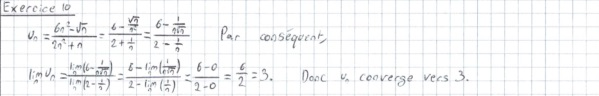
\includegraphics{ex10.jpg}
	
	\vspace{5mm}
	\noindent
	\textbf{Exercice 11.} Soit $(u_n) \in \mathbb{R}^{\mathbb{N}}$ une
	suite convergente.\\
	Montrer que $(\abs{u_n})$ est une suite convergente et
	\[\lim\limits_{n}\abs{u_n} = \abs{\lim\limits_{n}u_n}\]
	
	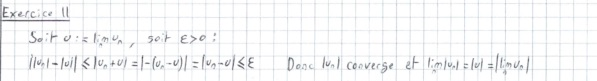
\includegraphics{ex11.jpg}
	
	\newpage
	
	\noindent
	\textbf{Exercice 12.}  Soit
	$(u_n)_{n \in \mathbb{N}} \in \mathbb{R}^{\mathbb{N}}$ une suite et
	$\ell \in \mathbb{R}$. Montrer que les assertions
	\[\forall \epsilon > 0, \exists N \in \mathbb{N}, \forall n \geq N,
		\abs{u_n - \ell} < \epsilon\]
	et
	\[\forall \epsilon > 0, \exists N \in \mathbb{N}, \forall n \geq N,
		\abs{u_n - \ell} \leq \epsilon\]
	sont équivalentes.
	
	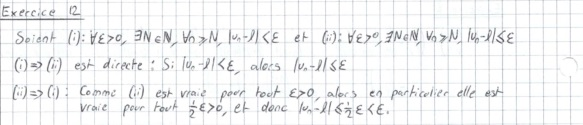
\includegraphics{ex12.jpg}
	
	\vspace{5mm}	
	\noindent
	\textbf{Exercice 13.} Déterminer le caractère de convergence de
	chacune des suites suivantes et calculer leur limite lorsqu'elle
	existe.
	\begin{enumerate}[label=(\roman*)]
		\item $a_n = \sqrt{n + 3} - \sqrt{n + 1}$ \\
		(Il est souvent utile de multiplier les expressions de la forme
		$\sqrt{A} - \sqrt{B}$ par $\sqrt{A} + \sqrt{B}$)
		%
		\item $\displaystyle b_n = (-1)^n \left(\frac{n + 5}{n}\right)$
		%
		\item $\displaystyle c_n = \frac{n(n-1)}{2^n - 5}$\\
		(On peut montrer que $2^n \geq n^3$ pour $n \geq 10$ en
		raisonnant par récurrence puis utiliser ce résultat).
		%
		\item $\displaystyle d_n = \left(\frac{2n^3}{n^3 - 7}\right)^2$
	\end{enumerate}
	
	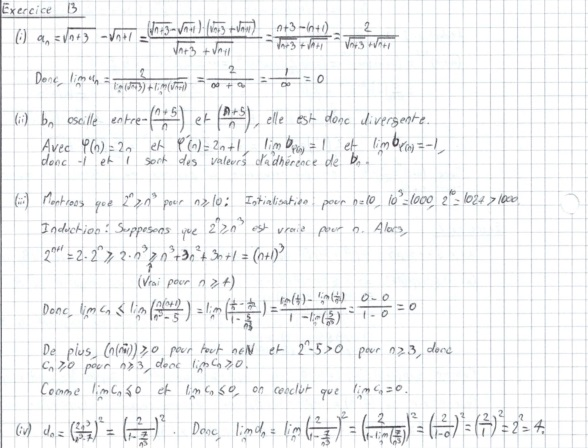
\includegraphics{ex13.jpg}
	
%	
%	
%	\colorbox{solution}
%	{
%		\begin{minipage}{0.9\textwidth}
%			s
%		\end{minipage}
%	}
%	
%	\colorbox{solution}
%	{
%		\begin{minipage}{0.9\textwidth}
%			\begin{enumerate}[label=(\alph*)]
%				\item a
%			\end{enumerate}
%		\end{minipage}
%	}
	
\end{document}
